\documentclass{beamer}

\usepackage[english]{babel}

\usepackage{appendixnumberbeamer}
\expandafter\def\expandafter\insertshorttitle\expandafter{%
  \insertshorttitle\hfill\insertframenumber\,/\,\inserttotalframenumber}
  
\usepackage{amsmath,amssymb,latexsym,amscd}
\usepackage{amsmath,amsfonts,amsthm} % Math packages
\usepackage{graphicx}
\usepackage{xcolor}
\usepackage{float} 			% para forzar a que las imagenes se queden en un lugar
\usepackage{enumerate}
\usepackage{amsthm}
\usepackage{array}
\usepackage{epstopdf}
\usepackage{ragged2e}		% para justificar
\usepackage{etoolbox}
\usepackage{multirow}
\usepackage{bibentry}
\usepackage{array}

\justifying

\theoremstyle{plain}

\apptocmd{\frame}{}{\justifying}{}
\apptocmd{\itemize}{}{\justifying}{}

\newcommand{\linea}{\noindent\makebox[\linewidth]{\rule{\textwidth}{1pt}}}

\newtheorem{thm}{Theorem}
\newtheorem{obj0}[thm]{Objetivo [v0]}
\newtheorem{obj1}[thm]{Objetivo [v1]}
\newtheorem{obj2}[thm]{Objetivo [v2]}
\newtheorem{simp}[thm]{Posibles simplificaciones}

\numberwithin{equation}{section} % Number equations within sections (i.e. 1.1, 1.2, 2.1, 2.2 instead of 1, 2, 3, 4)
\numberwithin{figure}{section} % Number figures within sections (i.e. 1.1, 1.2, 2.1, 2.2 instead of 1, 2, 3, 4)
\numberwithin{table}{section} % Number tables within sections (i.e. 1.1, 1.2, 2.1, 2.2 instead of 1, 2, 3, 4)

%\usetheme{Montpellier}
%\usetheme{Madrid}
%\usetheme{Marburg}
\usetheme{CambridgeUS}

\usecolortheme{whale}

\setbeamercolor{frametitle}{bg=gray,fg=white}
\setbeamertemplate{blocks}[rounded][shadow=false]
\setbeamercolor{block title}{use=structure,fg=black,bg=gray!15!white}
\setbeamercolor{block body}{use=structure,fg=black,bg=gray!5!white}

\input{macros.tex}

\begin{document}

%\renewcommand{\inserttotalframenumber}{\pageref{lastslide}}

\title[]{Classification of Musical Periods}
\author[Mauricio Toledo-Acosta]{Gerardo Mauricio Toledo Acosta\\
\medskip
{\small Postdoctorado\\ 
Laboratorio de Semántica Computacional\\
Centro de Investigación en Ciencias\\
UAEM
} 
}

\date{\today}

{\usebackgroundtemplate{
\includegraphics[width=\paperwidth]{BackgroundPS2.png}}
\maketitle }

%=====================================================================================



{
\usebackgroundtemplate{
\includegraphics[width=\paperwidth]{BackgroundPS2.png}}

\begin{frame}
\frametitle{Objetivo}

\uncover<1->{En la historia de la m\'usica hay varios periodos muy diferentes:}

\uncover<2->{
\begin{itemize}
\item Periodo barroco: 1600-1750.
\item Periodo cl\'asico: 1750-1820.
\item Periodo rom\'antico: 1820-1900.
\end{itemize}}

\uncover<3->{
\begin{obj0}
\justifying
?`Es posible clasificar la m\'usica en estos periodos usando una red neuronal?
\end{obj0}
}

\uncover<4->{
\begin{obj1}
\justifying
?`Es posible clasificar representaciones gr\'aficas de la m\'usica en estos periodos usando una red neuronal?
\end{obj1}
}

\end{frame}


\begin{frame}[label=enfoque]
\frametitle{2. ?`C\'omo abordar el problema?}
Dos enfoques:

\begin{itemize}
\justifying
\item Usando espectrogramas: mapas de calor de amplitud en el dominio de tiempo vs frecuencia.
\begin{figure}[H]
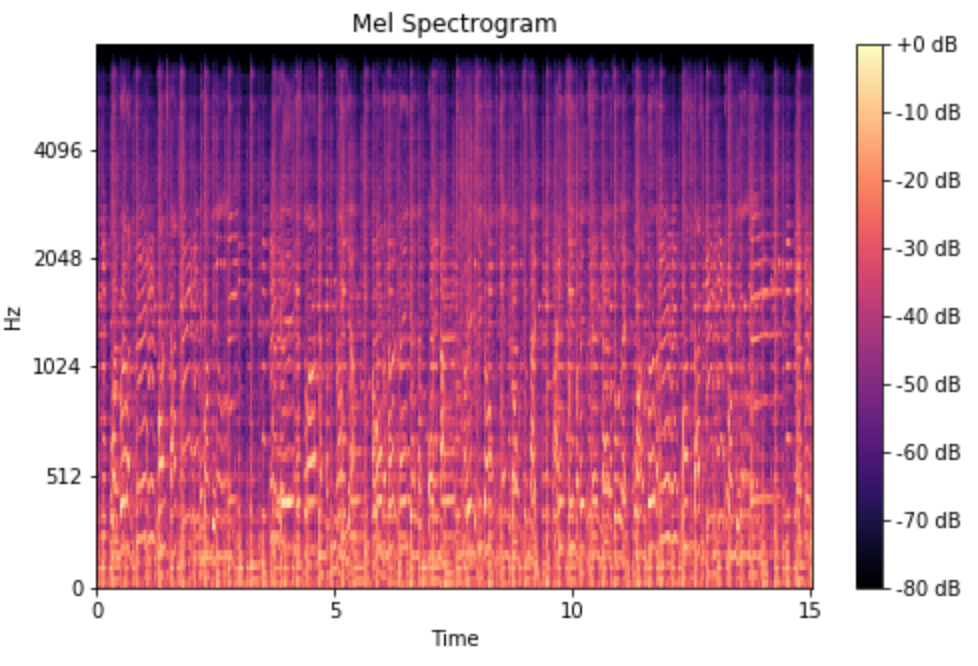
\includegraphics[height=22mm]{spectrogram.png}
\end{figure}

\item Usando secuencias midis: mapas de calor de amplitud en el dominio de tiempo vs notas tocadas.
\begin{figure}[H]
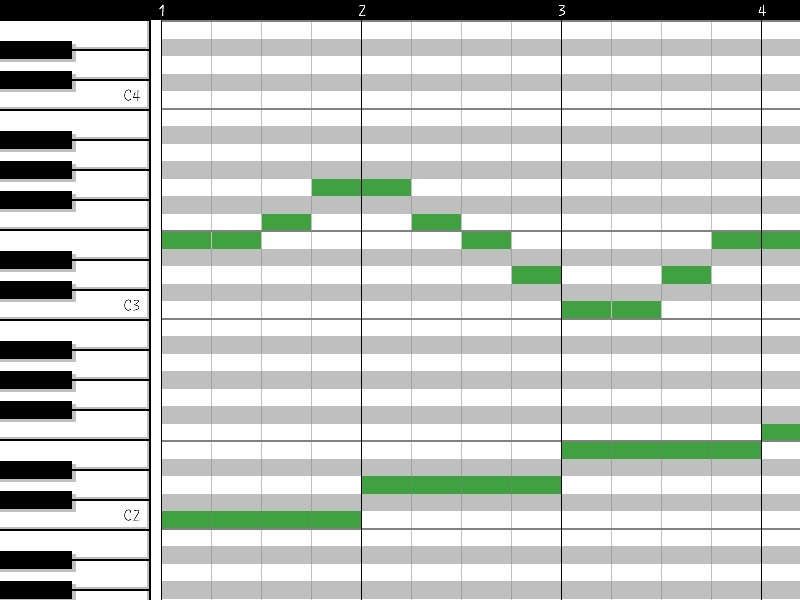
\includegraphics[height=20mm]{piano-roll.png}
\end{figure}
\begin{center}
\hyperlink{midi}{\beamerbutton{?`Qu\'e es un archivo midi?}}
\end{center}

\end{itemize}

\end{frame}

%----------------------------------------


\begin{frame}
\frametitle{2. ?`C\'omo abordar el problema?}
\justifying

\begin{table}[h!]

\begin{center}
\begin{tabular}{p{0.45\textwidth} | p{0.45\textwidth}}
\justifying
\uncover<1->{
Tengo un dataset de 1549 
archivos midi de piezas de piano de los tres periodos.} &

\uncover<2->{
Origen: Kaggle, The MAESTRO Dataset (Tensorflow), websites de midis.} 
\end{tabular}
\end{center}
\end{table}


\uncover<3->{
He generado un piano-roll de cada archivo midi:

\begin{table}[h!]
\begin{center}
\begin{tabular}{ccc}

Barroco & Cl\'asico & Rom\'antico \\

\begin{minipage}{.3\textwidth}
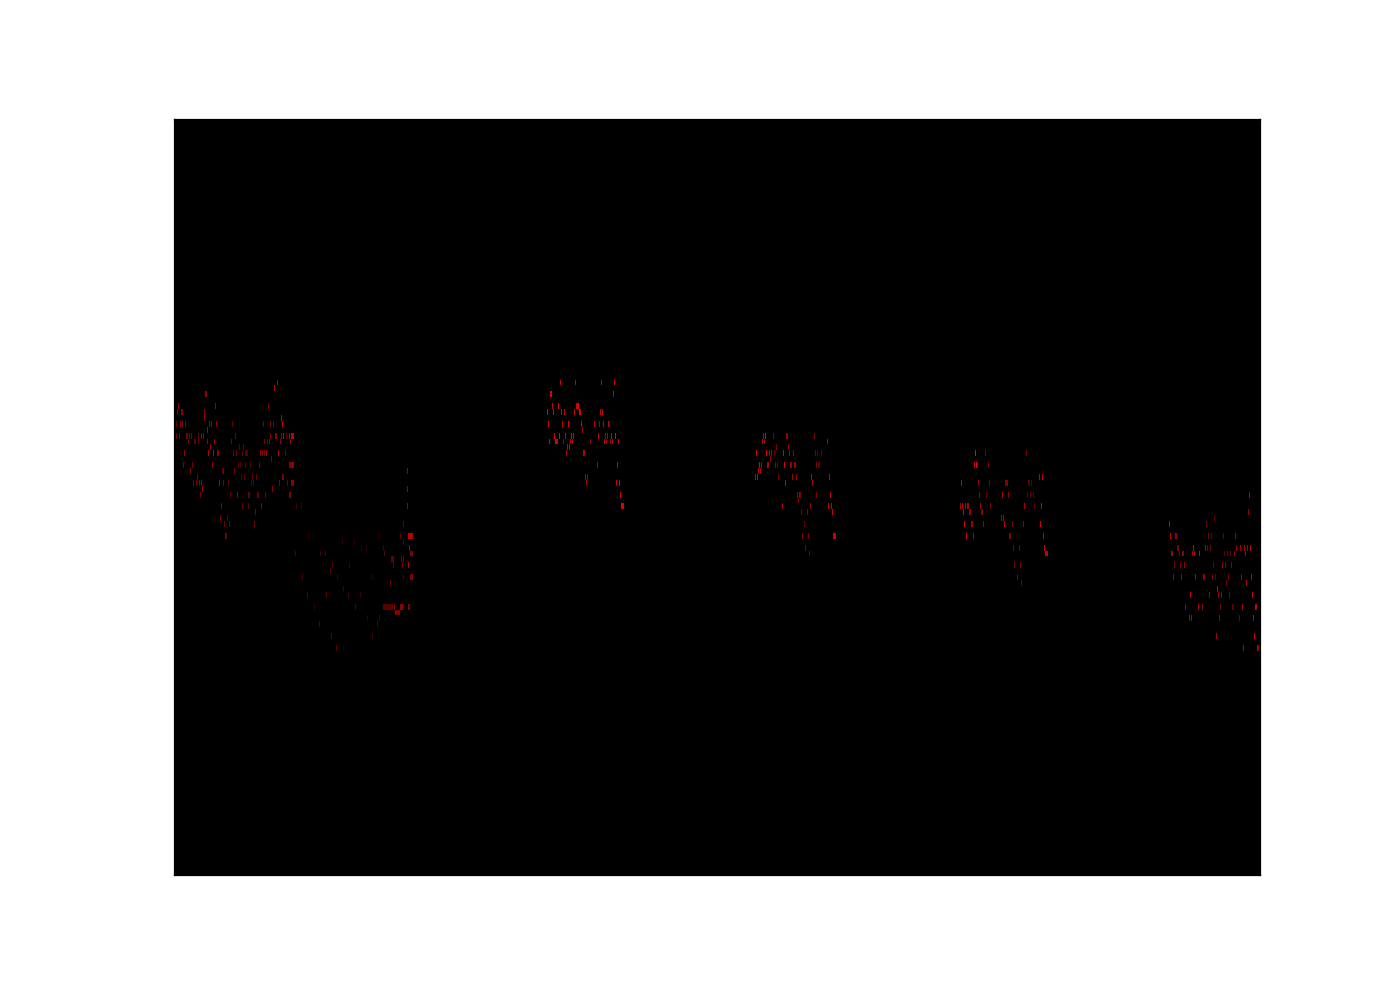
\includegraphics[width=\linewidth, height=25mm]{1barroco.png}
\end{minipage}

 &
\begin{minipage}{.3\textwidth}
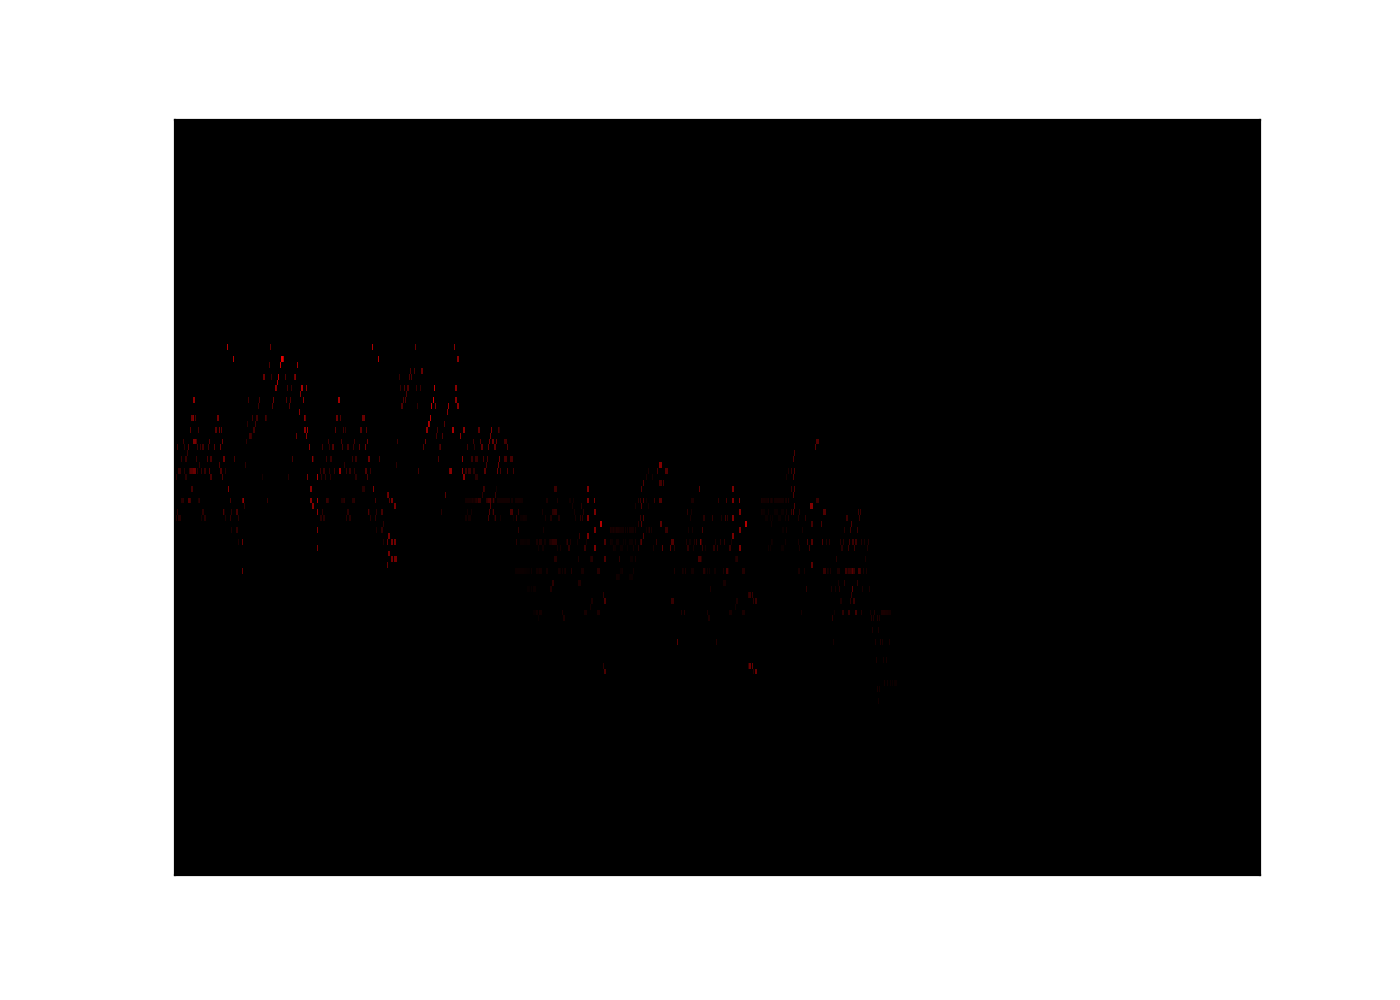
\includegraphics[width=\linewidth, height=25mm]{2clasico.png}
\end{minipage}

&

\begin{minipage}{.3\textwidth}
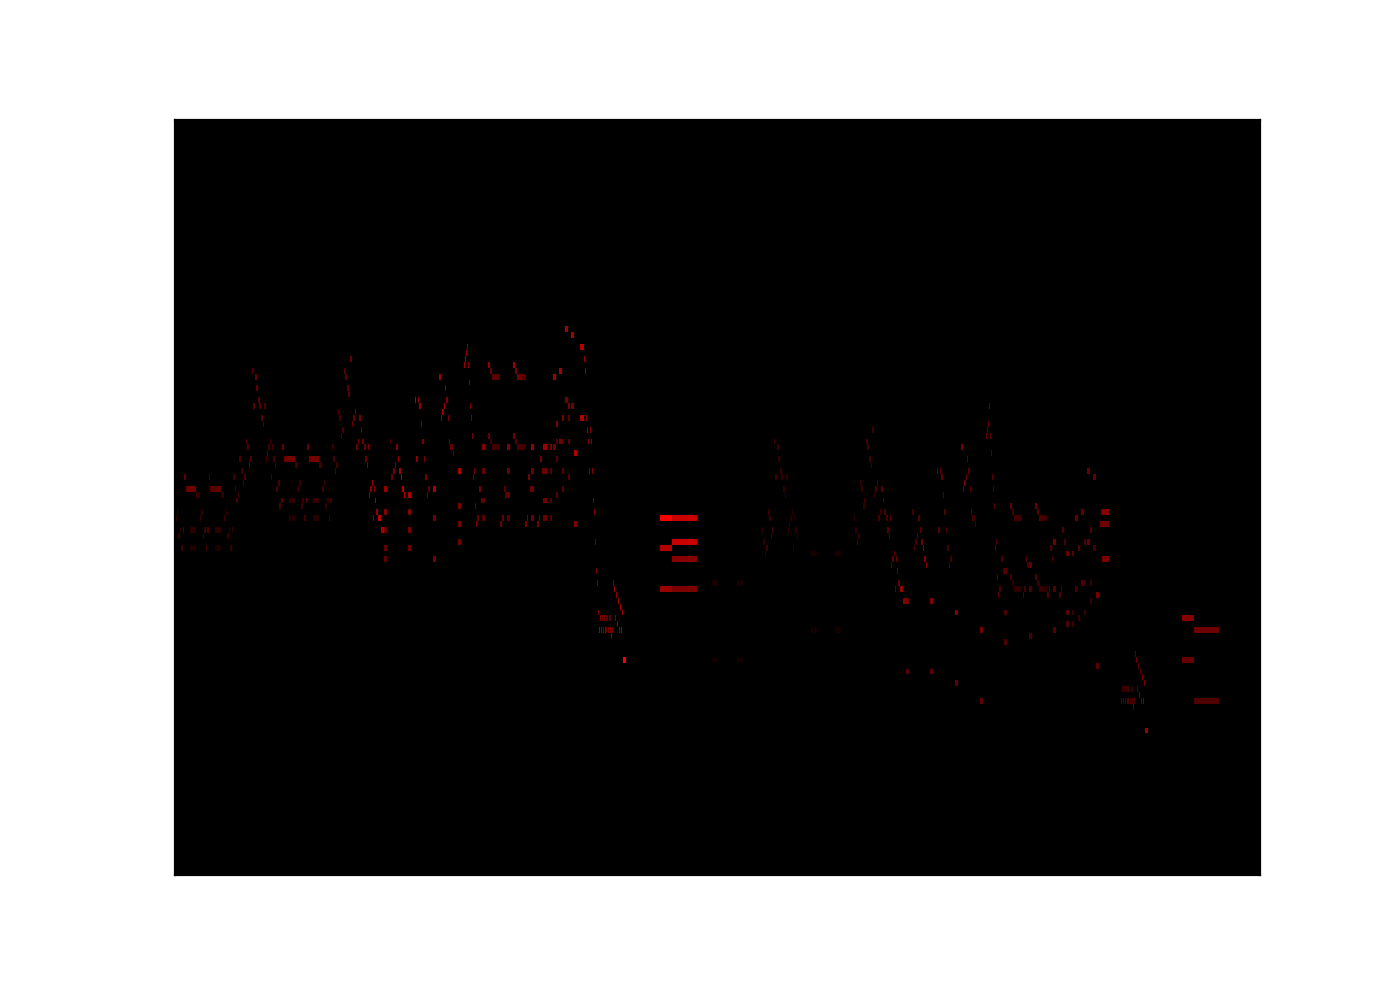
\includegraphics[width=\linewidth, height=25mm]{3romantico.png}
\end{minipage}


\\
\end{tabular}
\end{center}
\end{table}

}


\uncover<4->{
\begin{obj2}
Entrenar una red neuronal para clasificar las imagenes.
\end{obj2}
}
\end{frame}

%----------------------------------------


\begin{frame}
\frametitle{Posibles dificultades derivadas del dataset}
\justifying

\begin{itemize}[<+->]
\item No son tantas instancias.

\item Tama\~nos relativos desproporcionados
\begin{figure}[H]
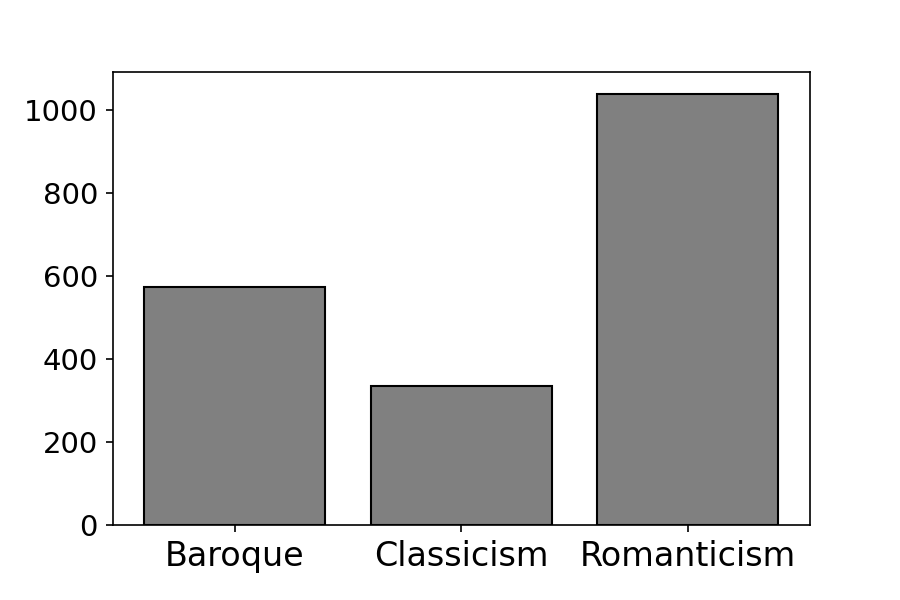
\includegraphics[height=27mm]{histogram_periods.png}
\end{figure}


\item Configuraci\'on correcta de los par\'ametros de las imagenes.

\end{itemize}

\end{frame}

%----------------------------------------

\begin{frame}
\frametitle{Posibles dificultades derivadas del problema}
\justifying

\begin{itemize}[<+->]
\item Hay traslapses entre los periodos.
\medskip
\item Diferencias de estilos entre compositores del mismo periodo.
\end{itemize}
\medskip

\bigskip

\uncover<3->{
\begin{simp}
\begin{itemize}[<+->]
\item Clasificar entre dos periodos solamente.
\item Clasificar entre compositores.
\end{itemize}
\end{simp}
}

\end{frame}

%===========================================================================================================
%===========================================================================================================
\appendix

\section{Appendix}


\begin{frame}[label=midi]
\frametitle{?`Qu\'e es un archivo midi?}
\justifying

Un archivo midi almacena una secuencia de notas, indicando su frecuencia, tiempo de activaci\'on, tiempo de finalizaci\'on, intensidad de la nota. Adem\'as de informaci\'on de la pieza o canci\'on.\\

\medskip

Consta de mensajes de la forma:\\

\begin{figure}[H]
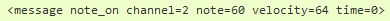
\includegraphics[height=5mm]{midi-msg.png}
\end{figure}



\hyperlink{enfoque}{\beamerbutton{Regresar}}
\end{frame}


}

\end{document}